%%%%%%%%%%%%%%%%
\section{Control Solution}
\begin{frame}{Control Solution}{}
    \centering
    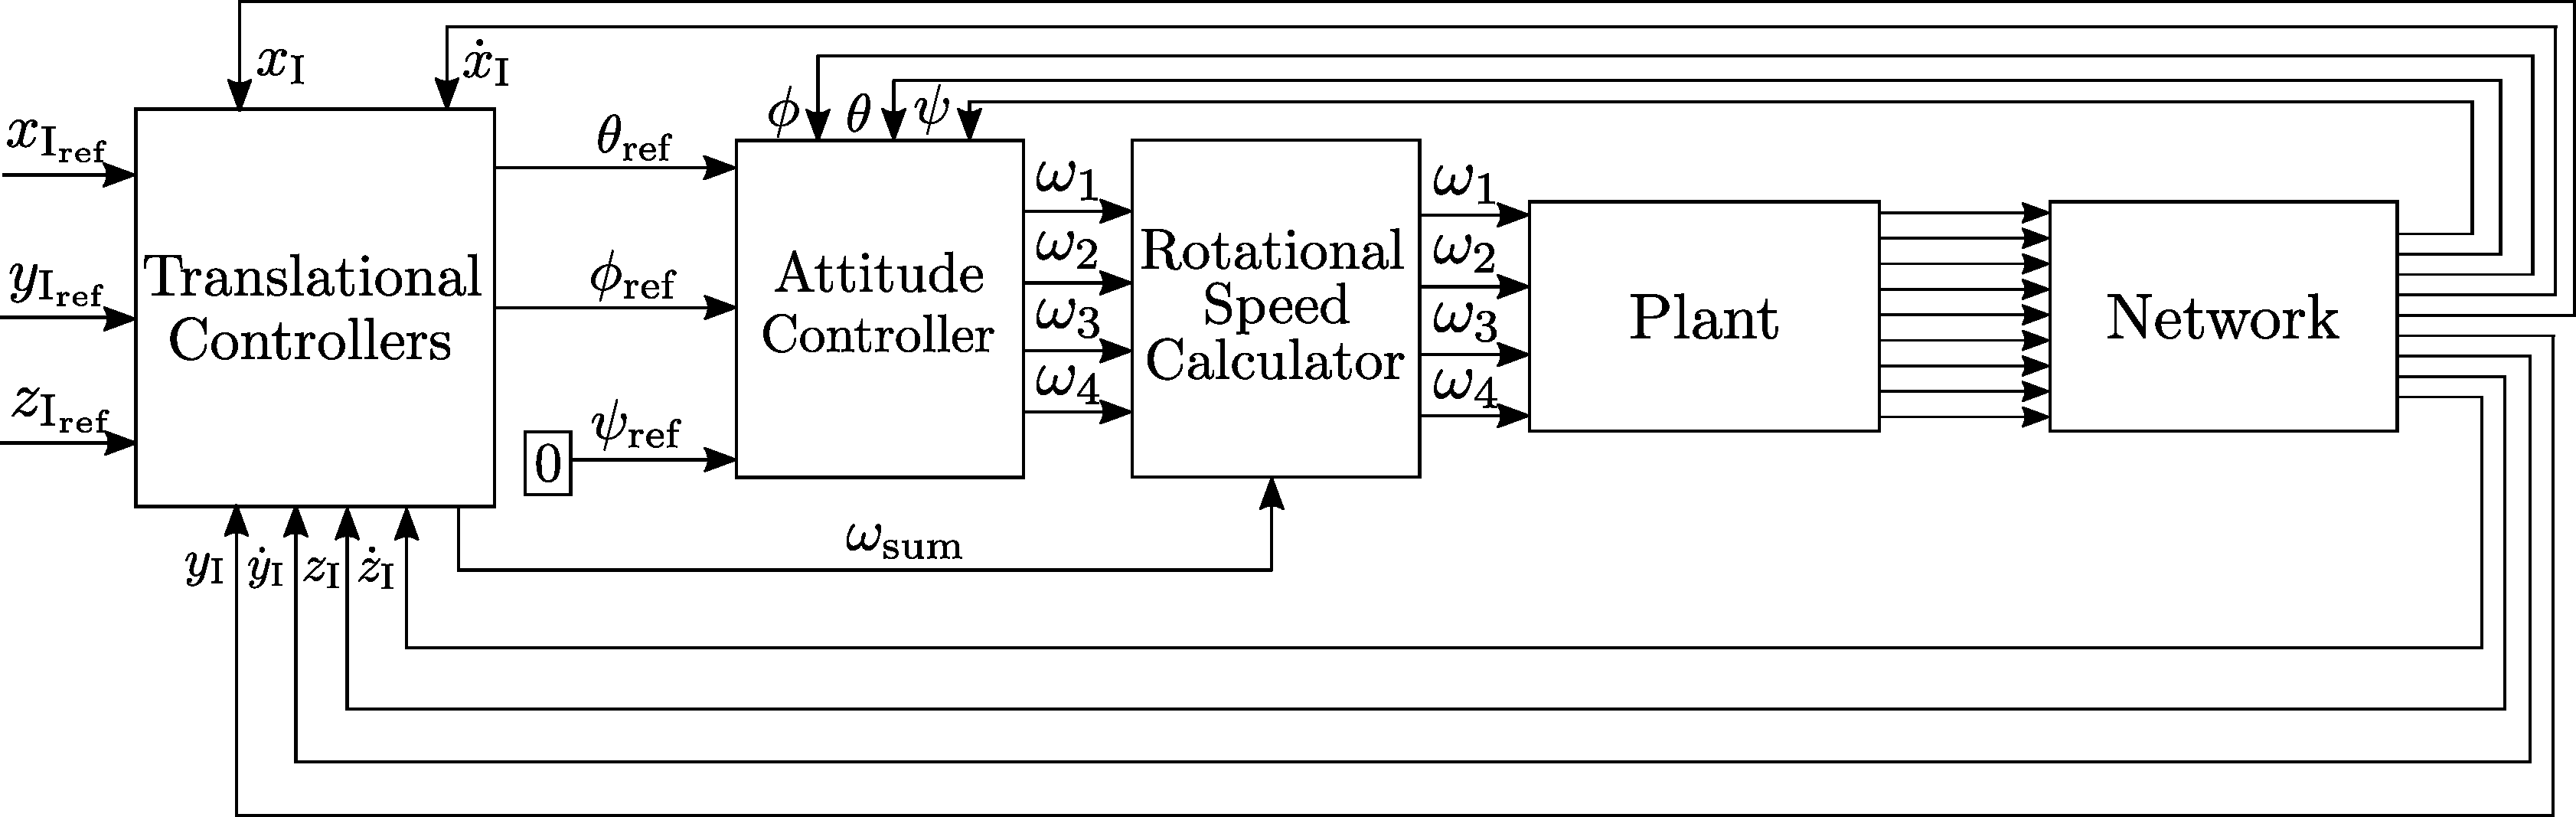
\includegraphics[scale=0.2]{figures/ControlDiagramPoster}
\end{frame}

\subsection{Attitude Controller}
\begin{frame}{Control Solution}{Attitude Controller}
    \centering
    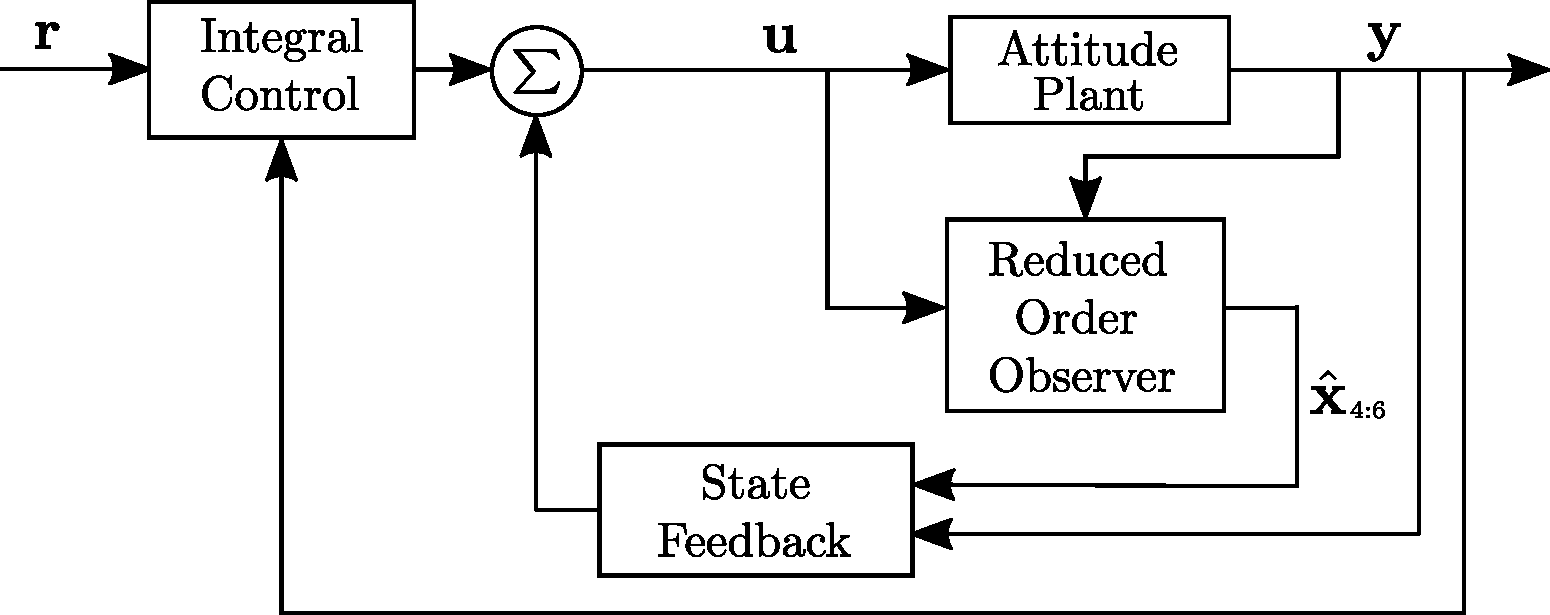
\includegraphics[scale=0.35]{figures/AttitudeControlDiagram}    
\end{frame}

\begin{frame}{Control Solution}{Attitude Controller}
    \begin{itemize}
        \item System Representation
    \end{itemize}

\begin{minipage}{\linewidth}
    \begin{minipage}{0.40\linewidth}
        \begin{flalign}
        \dot{\vec{x}}(t)&=\vec{A}\vec{x}(t) + \vec{B}\vec{u}(t) \nonumber \\
        \vec{y}(t)&=\vec{C}\vec{x}(t) \nonumber
        \end{flalign}
    \end{minipage}
    \hspace{0.03\linewidth}
    \begin{minipage}{0.55\linewidth}
        \begin{figure}[H]
            \includegraphics[width=1\textwidth]{figures/ABC}
        \end{figure}
    \end{minipage}
\end{minipage}

\begin{minipage}{0.22\linewidth}
    \begin{flalign}
    \vec{x} = 
    \begin{bmatrix}
    \phi \\
    \theta \\ 
    \psi \\
    \dot{\phi} \\
    \dot{\theta} \\
    \dot{\psi} \\
    \end{bmatrix}	\nonumber
    \end{flalign}  
\end{minipage}\hfill
\begin{minipage}{0.22\linewidth}
    \begin{flalign}
    \vec{u}= 
    \begin{bmatrix}
    \omega_1 \\
    \omega_2 \\
    \omega_3 \\
    \omega_4 \\
    \end{bmatrix} \nonumber
    \end{flalign} 
\end{minipage}\hfill 
\begin{minipage}{0.22\linewidth}
    \begin{flalign}
    \vec{y} = 
    \begin{bmatrix}
    \phi \\
    \theta \\ 
    \psi \\
    \end{bmatrix}	\nonumber
    \end{flalign}
\end{minipage}\hfill 
\end{frame}


\begin{frame}{Control Solution}{Attitude Controller}
    \begin{itemize}
        \item State Feedback with Integral Control
    \end{itemize}
    
    \begin{figure}
        \centering
        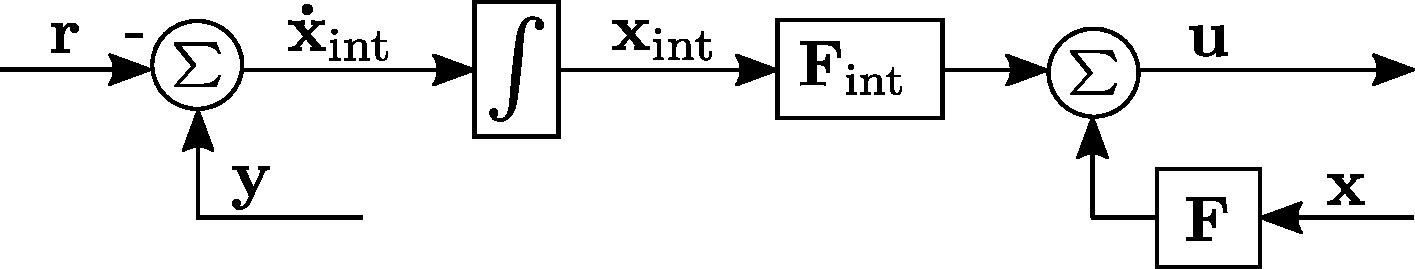
\includegraphics[scale=0.35]{figures/DetailedControllerColorDiagram}  
    \end{figure}
    \begin{flalign}
        \dot{\vec{x}}_{\mathrm{Int}}(t) &= \vec{y}(t)-\vec{r}(t)\nonumber
    \end{flalign}         
    \begin{flalign} 
    \vec{u}(t) &=\vec{F}  \vec{x}(t) + \vec{F}_{\mathrm{Int}}  \vec{x}_{\mathrm{Int}}(t) \nonumber
    \end{flalign}
\end{frame}

\begin{frame}{Control Solution}{Attitude Controller}
    \begin{itemize}
        \item LQR
    \end{itemize}
    \begin{flalign} 
        \cal{J} &= \int_{0}^{\infty} \vec{x}^T \vec{Q} \vec{x} + \vec{u}^T \vec{R} \vec{u} \ dt \nonumber
    \end{flalign}
     \begin{itemize}
         \item Bryson's Rule
     \end{itemize}   
    \begin{flalign} 
    Q_{ii} &= \frac{1}{\text{maximum acceptable value of }[x^2_i]}\nonumber\\
    R_{ii} &= \frac{1}{\text{maximum acceptable value of }[u^2_i]}\nonumber
    \end{flalign}
    
\end{frame}

\begin{frame}{Control Solution}{Attitude Controller}
    \begin{itemize}
        \item Reduced Order Observer
    \end{itemize}

    \begin{figure}[H]
        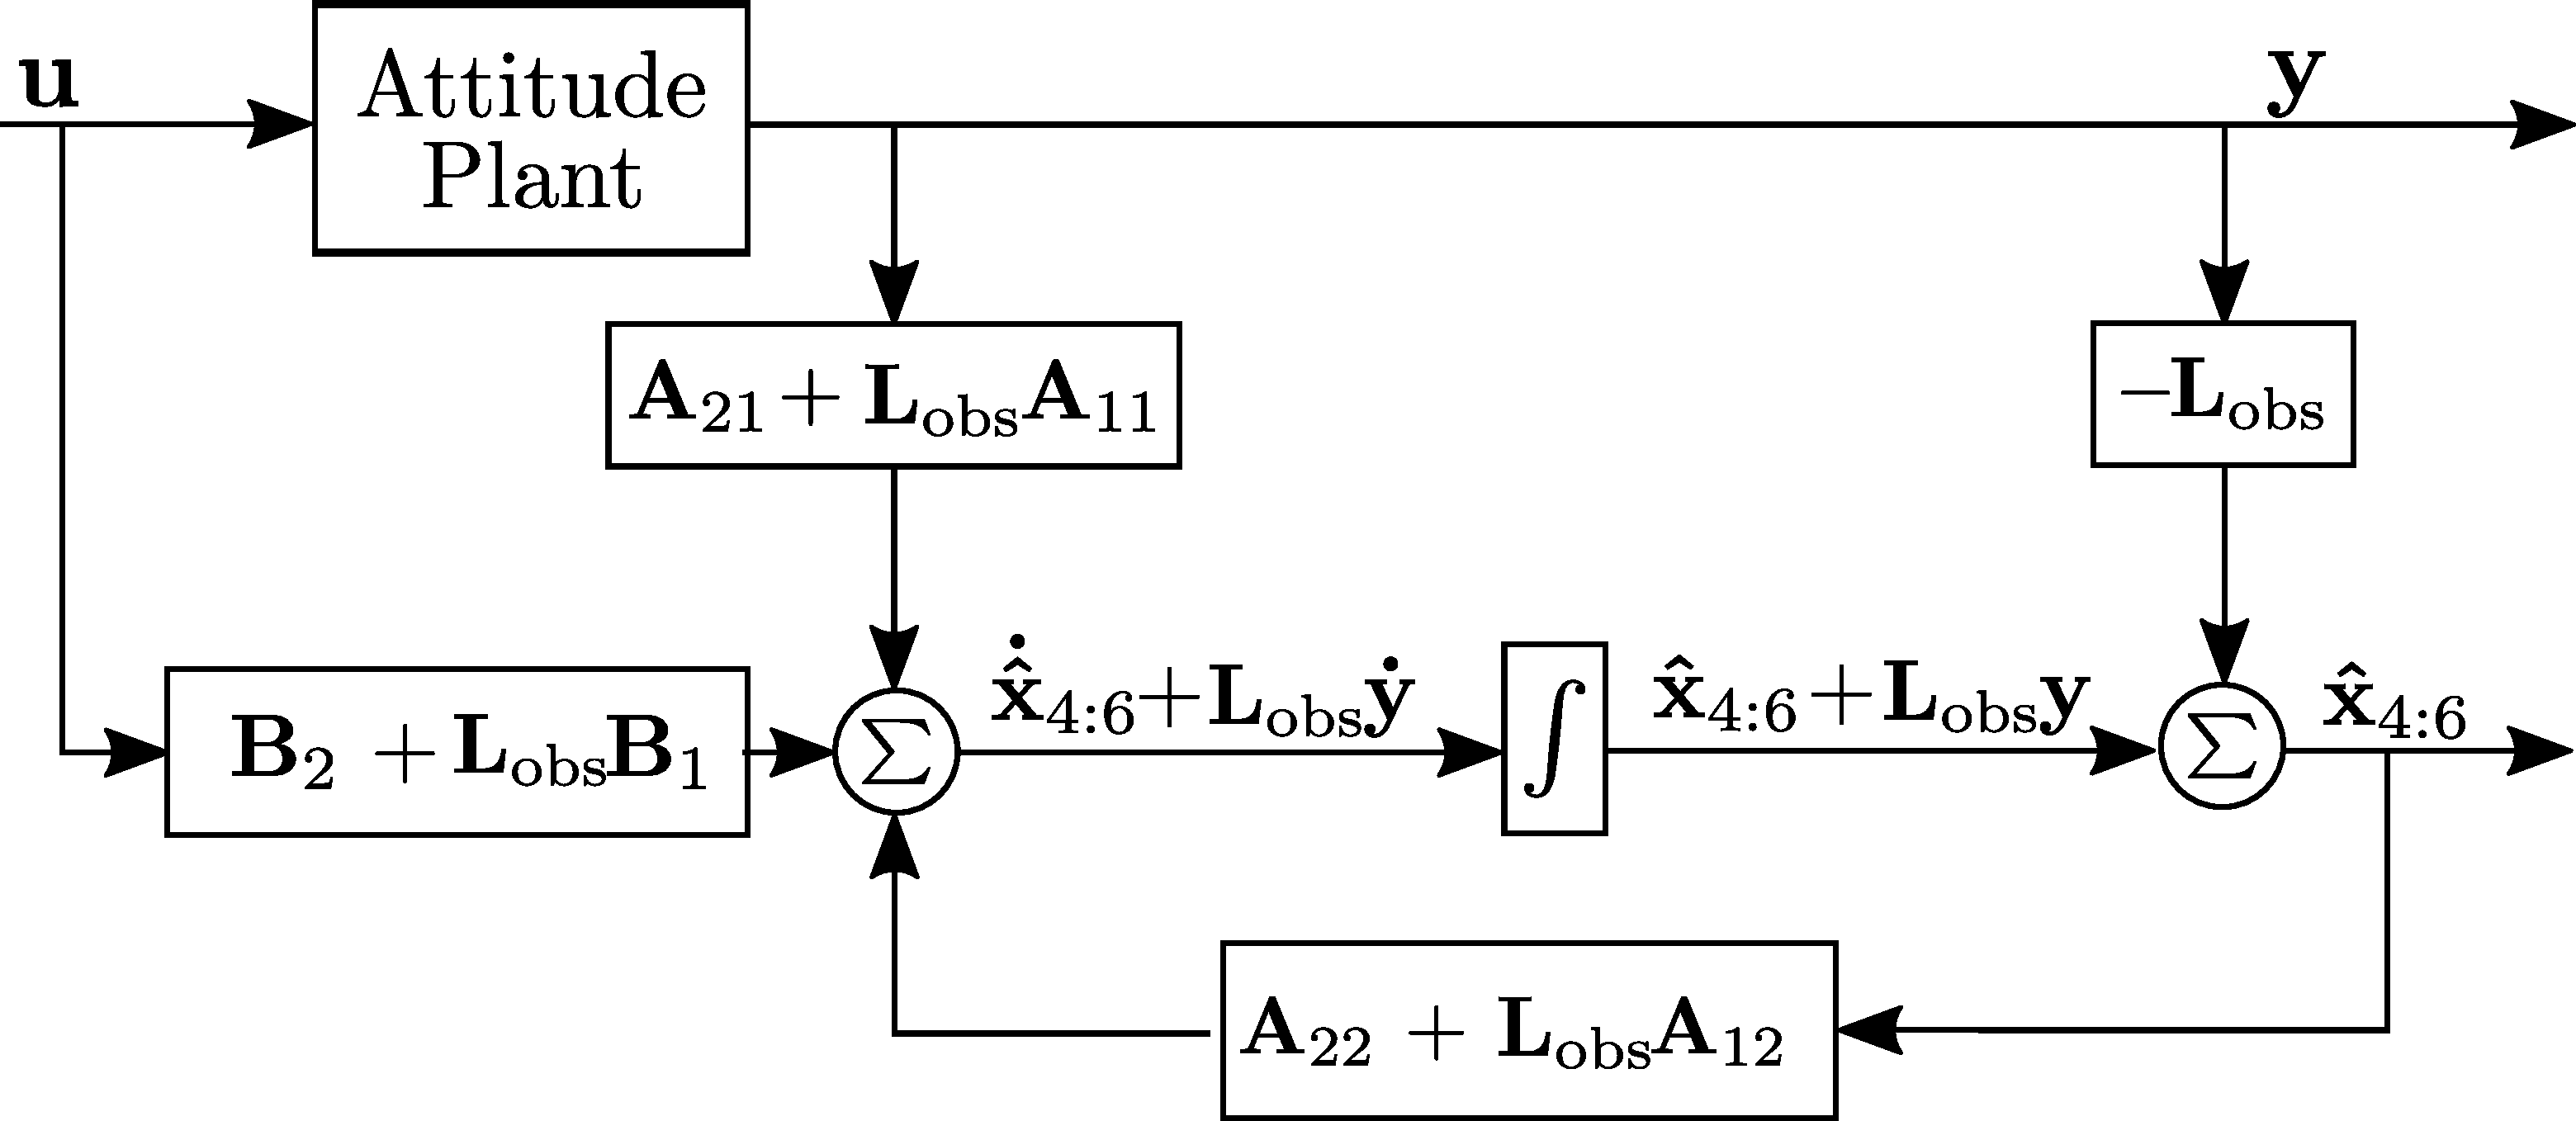
\includegraphics[width=0.6\textwidth]{figures/observerDiagram}
    \end{figure}

    \begin{minipage}{\linewidth}
        \begin{minipage}{0.49\linewidth}
            \begin{flalign}
            \vec{x}_\mathrm{4:6} = 
            \begin{bmatrix}
            \dot{\phi} \\
            \dot{\theta} \\
            \dot{\psi} \\
            \end{bmatrix}	\nonumber
            \end{flalign} 
        \end{minipage}
        \hspace{0.03\linewidth}
        \begin{minipage}{0.49\linewidth}
               \begin{flalign}
               \vec{A_{22}} + \vec{L_{obs}}\vec{A_{12}} \nonumber
               \end{flalign}                  
        \end{minipage}
    \end{minipage}

\end{frame}

%%
% TOC
\begin{frame}{Agenda}{}
    \tableofcontents
\end{frame}

%%